\documentclass[10pt]{exam}
\usepackage[hon]{template-for-exam}
\usepackage{graphicx}
\usepackage{tikz}
\usetikzlibrary{shadings,decorations.pathmorphing,arrows.meta}


\title{Projectile Motion PhET Simulation}
\author{Rohrbach}
\date{\today}

\begin{document}
\maketitle


\noindent
Go to the Projectile Motion PhET Simulation.  The link is on Schoology, or you can go to the website \texttt{https://phet.colorado.edu/} and type ``\texttt{Projectile Motion Intro}'' into the search bar.

\begin{itemize}
  \item Click ``Intro'' once it opens.

  \item Drag the cannon to the ground (altitude of 0 m)
  
    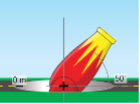
\includegraphics{altitude.png}

  \item Make sure to check the two boxes under Velocity Vectors.
  
    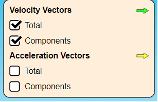
\includegraphics{checkboxes.png}
    
\end{itemize}



\begin{questions}
  
\question
  Fire the cannon.  Which method of vector addition is the simulation using (parallelogram or tip-to-tail)?
  \vs

\question
  When you fire the cannon, what happens to the $x$- and $y$- components of the vector over time?
  \vs

\question
  Increase and decrease the initial speed. How are the range (that is, how far across the ground) and height (that is how far in the air) affected by changing the initial speed? Why do you think this is?
  \vs

\pagebreak

\question
  Now change the angle. \label{angles}

  \begin{parts}
    \part
      Which angle has the tallest height?
      \vs

    \part
      Which angle has the longest range?
      \vs

    \part
      Why do you think this is?
      \vs[2]
      
  \end{parts}

\question
  Find pairs of angles that give the same range.  Find as many as you can.  See if you can notice a pattern.
  \vs[3] \label{pairs}

\question
  Explain the reason why your answers to \#\ref{angles} and \#\ref{pairs} make sense.  Your instructor will help you with this.
  \vs[3]



  \begin{tikzpicture}[red, very thick, ->]
    \draw (0,0) -- ++(30:5);
    \draw (6,0) -- ++(45:5);
    \draw (12,0) -- ++(60:5);

  \end{tikzpicture}

\end{questions}


\end{document}